\chapter{対話型数値計算}

本章の目的は、
Pythonの対話型実行環境であるJupyter-notebookを用いてコンピュータによる数値計算を体感し、プログラミングの原理を実感することである。

Jupyter-notebookは、簡単にデータ解析を実施し、その結果を再利用しやすく、かつ配布しやすい形で残すことができるため、現在急激に利用が広まっているソフトウェアである。

インストールも簡単であるため、各自のPCにもインストールすることを勧める。詳しくは、\ref{chap:anaconda}章を参照すること。

\section{Jupyter-notebookの起動}
Jupyte起動するためにコマンドプロンプトを実行する。
いくつか方法があるが「Winキー」+「R」を同時押しして「ファイル名から起動」を実行し、

\url{cmd}

\noindent を入力しEnterを押す方法が簡単である(図\ref{fig:Anaconda_launch1})。
コマンドプロンプトで

\url{Jupyter-notebook}

\noindent を入力し実行すると(図\ref{fig:Anaconda_launch2})、
Jupyter-notebookのスタート画面が立ち上がる(図\ref{fig:Anaconda_launch3})。
 
\begin{figure}
	\centering
	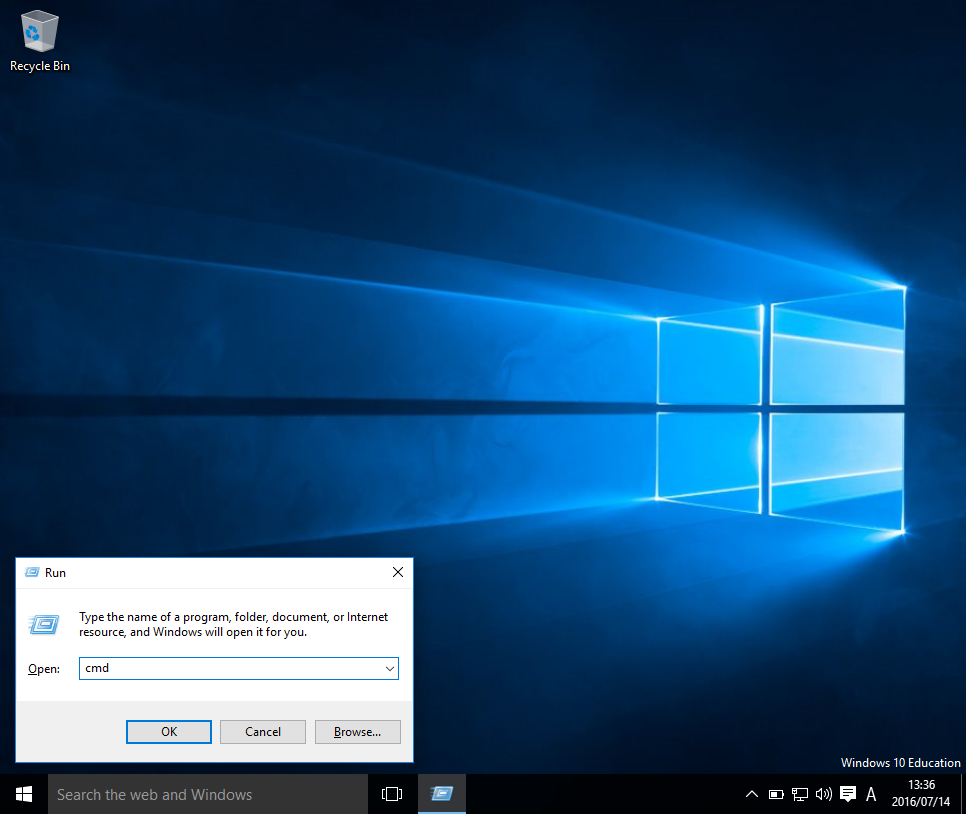
\includegraphics[width=10cm]{TeX_files/fig_python_install/Anaconda_launch1.png}
	\caption{
		\label{fig:Anaconda_launch1}
		「Winキー」+「R」を押して出てくる検索窓に「cmd」を入力してEnterを押す。
			}
\end{figure}

\begin{figure}
	\centering
	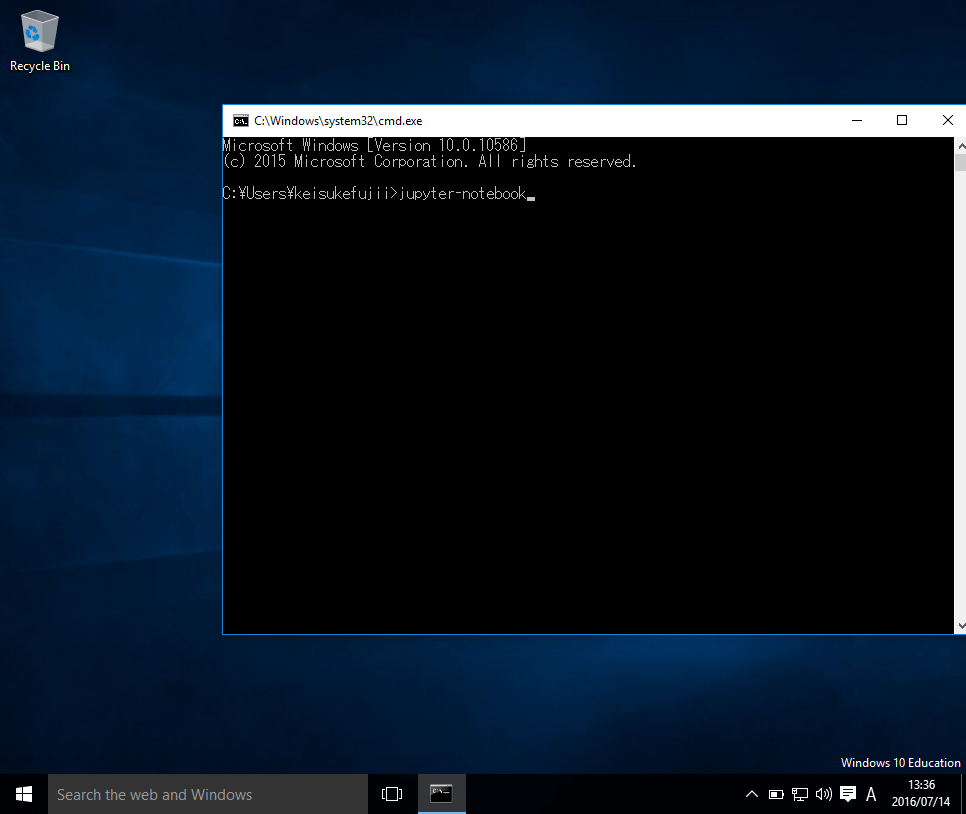
\includegraphics[width=10cm]{TeX_files/fig_python_install/Anaconda_launch2.png}
	\caption{
		\label{fig:Anaconda_launch2}
		コマンドプロンプト内で「Jupyter-notebook」と入力し実行する。
	}
\end{figure}

\begin{figure}
	\centering
	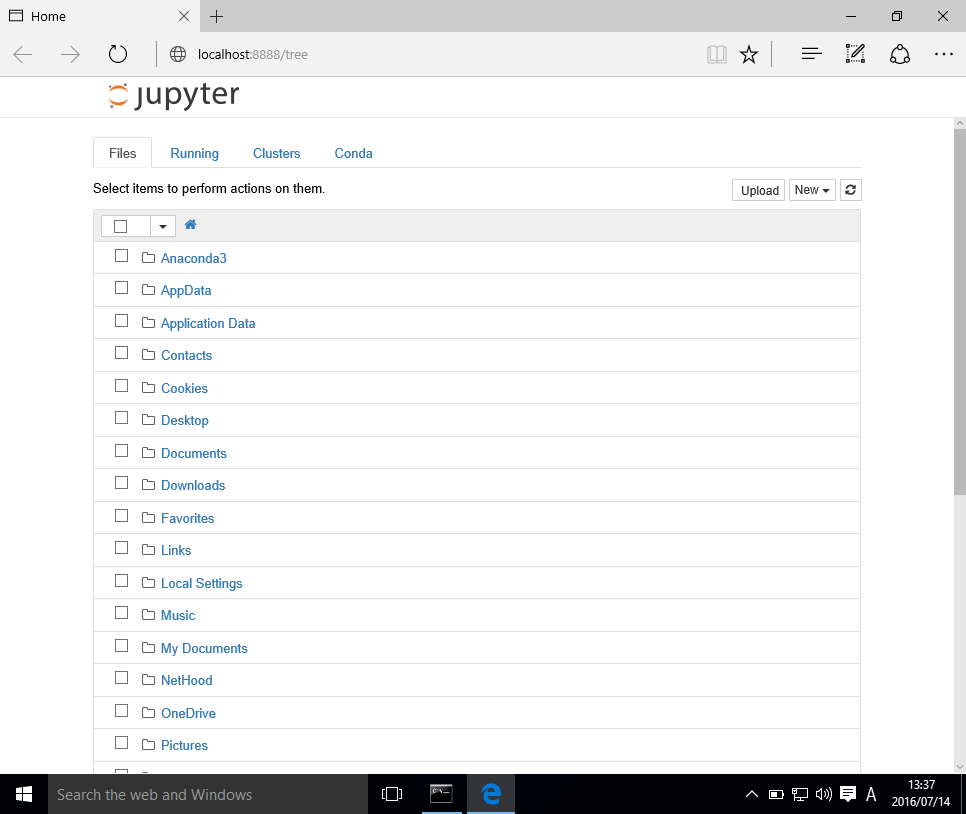
\includegraphics[width=10cm]{TeX_files/fig_python_install/Anaconda_launch3.png}
	\caption{
		\label{fig:Anaconda_launch3}
		Jupyter-notebookの起動画面の一例。
	}
\end{figure}

\section{Jupyer-notebookファイルの作成}
これからJupyter-notebookファイルを大量に作成することになる。
作成したファイルを見つけやすくするために、フォルダ構造を整理する。

マイドキュメント フォルダの中に、Johokisoenshuフォルダを作成する。
そのため、マイドキュメントフォルダをクリックしたあと、NewボタンからFolderをクリックする。
作成したフォルダの左側のチェックボックスをクリックすると出てくる renameボタンを押すことで名前の変更ができる(図\ref{fig:Jupyter_launch1})。

Johokisoenshuフォルダ内に移動し、NewボタンからPython 3を起動する。
新しいウィンドウが開く(図\ref{fig:Jupyter_launch2})。

新しいノートブックファイルには名前がまだつけられていないので、名前を変更する。
Jupyerロゴの横のUntitledをクリックすることで名を変更できる。
今日は演習の1日目なのでEnshu1とする(図\ref{fig:Jupyter1})。


\begin{figure}
	\centering
	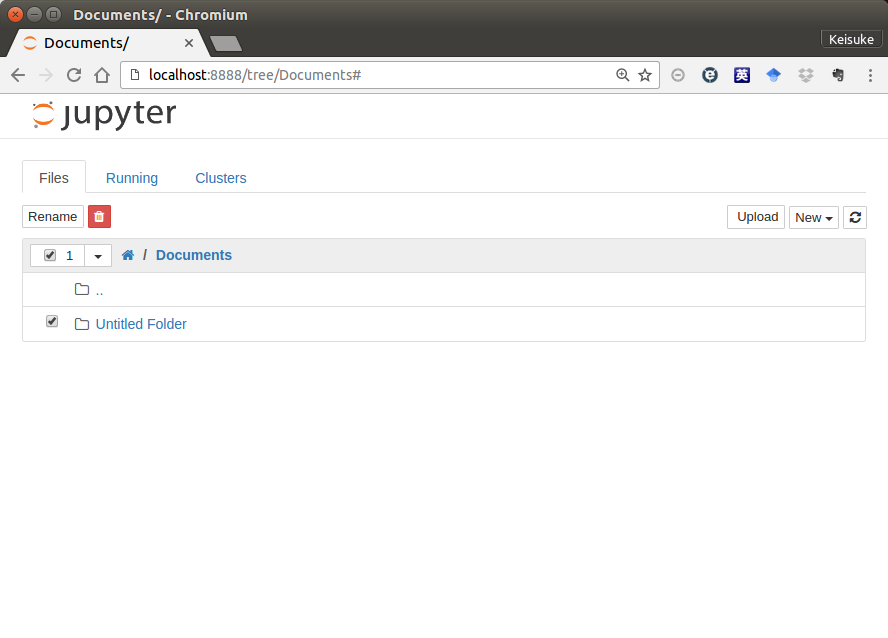
\includegraphics[width=10cm]{TeX_files/fig_python_install/Jupyter-launch1.png}
	\caption{
		\label{fig:Jupyter_launch1}
		Jupyter-notebookでフォルダ構造を整理する。フォルダ名左横のチェックボックスを押すと、\tt{rename}ボタンが出てくる。
	}
\end{figure}

\begin{figure}
	\centering
	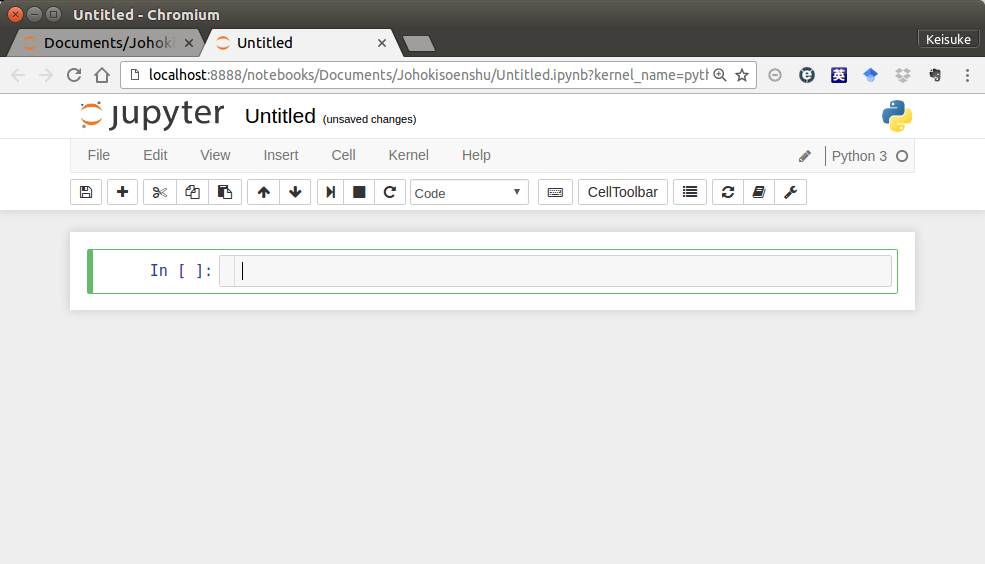
\includegraphics[width=10cm]{TeX_files/fig_python_install/Jupyter_launch2.png}
	\caption{
		\label{fig:Jupyter_launch2}
		Jupyter-notebookで新しいPythonノートブックファイルを作成したときの様子。
	}
\end{figure}

\begin{figure}
	\centering
	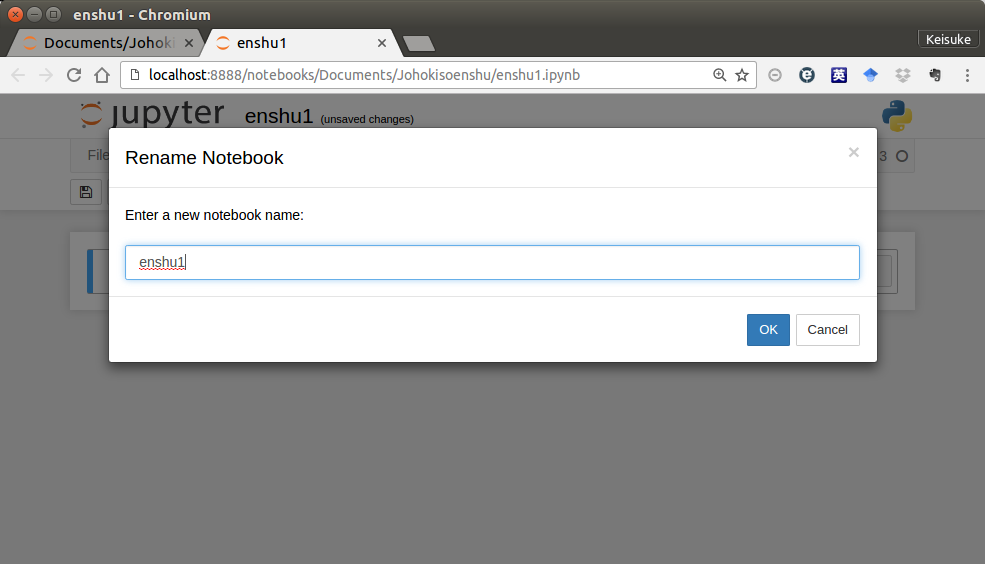
\includegraphics[width=10cm]{TeX_files/fig_python_install/Jupyter1.png}
	\caption{
		\label{fig:Jupyter1}
		Jupyter-notebookファイルの名前を変更する。
	}
\end{figure}

\section{Jupyter-notebookの終了}
Jupyter-notebookを終了するためには、コマンドプロンプドでCtrl+Cを押す。